\chapter{Potvrzení simulace}
\label{chap:sim_confirmation}

Po navržení a implementaci simulace je dalším krokem sledování její přesnosti a porovnání s reálnými experimenty. První způsob porovnání již byl zmíněn v \autoref{chap:drag}, kde jsme porovnávali simulované a reálné dopady tření na spinner, a to bez externího magnetického pole (viz \autoref{fig:drag_fit}, \autoref{fig:drag_fit_wlin}) i v externím magnetickém poli (viz \autoref{fig:drag_fit_mag}, \autoref{fig:drag_fit_mag_wlin}). Všechna tato měření byla prozatím velmi podobná našim simulovaným hodnotám, ale byl použit pouze jeden spinner. Další experimenty se tedy zaměří na další okrajové případy a použití více spinnerů.

\section{Vysokorychlostní video}

Nevýhodou minulého měření pomocí magnetického čidla Vernier je, že jsme nebyli schopni přesně určit okamžitou pozici a rychlost. Toto nebyl tak velký problém, jelikož náš celkový záznam byl velmi dlouhý a nezajímalo nás mikroskopické chování spinneru, ale spíše makroskopický dopad tření na jeho schování. Nyní však budeme sledovat okamžité chování spinneru pomocí trackování videa natočeného vysokorychlostní kamerou. K trackování použijeme volně dostupný software zvaný \texttt{Tracker} \cite{Tracker}. Snímkovou frekvenci jsme nastavili v jednom experimentu na 60 snímků za sekundu, ve zbylých experimentech na 1000 snímků za sekundu.

\subsection{Aparatura}

\begin{wrapfigure}{r}{0.40\textwidth}
    % \vspace*{0.75cm}
    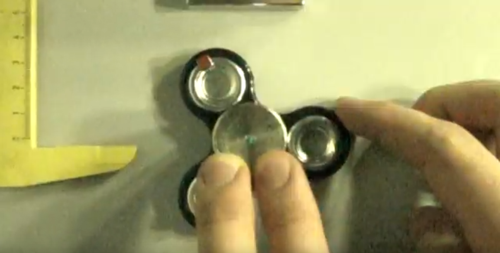
\includegraphics[width=0.40\textwidth]{slowmo_aparature_ss2.png}
    \centering
    \caption{Snímek ze záznamu jednoho z experimentů}
    \label{fig:slowmo_aparature_ss2}
\end{wrapfigure}

Aparatura pro následující experimenty je relativně jednoduchá. Jeden spinner osazený magnety je umístěn pevně na vodorovnou podložku a jeden z magnetů je barevně označen, abychom ho mohli trackovat. Ve vzdálenosti 8cm od něj je ve stejné rovině umístěn velký magnet (jehož remanenci jsme změřili v \autoref{sec:remanence_measurement}) a směr jeho magnetického momentu je kolmo vzhůru (stejně jako u magnetů spinneru). Celý systém je poté snímán kamerou umístěnou kolmo nad středem spinneru.

\subsection{Proces trackování}

Proces trackování videa je značně usnadněn schopností softwaru \texttt{Tracker} vyhledávat značky automaticky pomocí definované vyhledávací masky. Pokud \texttt{Tracker} není schopen s dostatečnou jistotou pozici značky ve videu najít, musí být doplněna manuálně. Z trackovaných dat pozice značky v čase jsme poté schopni jednoduše dopočítat, pod jaký úhlem se spinner nachází v daný moment. Z rozdílů dvou úhlů jsme také schopni dopočítat přibližnou okamžitou úhlovou rychlost.

\subsection{Výsledky měření při 60fps}

První měření, označené C0000, je měření prováděné při snímkovací frekvenci 60 fps\footnote{Jednotka \textbf{fps}, vycházející z anglického \textit{frames per second}, je často používaná zkratka pro českou jednotku "snímky za sekundu".}.
Nižší snímkovací frekvenci jsme si vybrali, jelikož naše kamera není schopna na vyšší frekvenci natáčet déle než 2 sekundy. Účelem tohoto experimentu bylo určit, do jaké míry se výsledky naší simulace a měření rozchází po uplynutí většího časového úseku. Spinner má kvůli působení vnějšího magnetu rovnovážnou polohu, ze které je v tomto experimentu vychýlen a poté ponechán oscilovat.

\begin{figure}[!ht]
    % \vspace*{0.75cm}
    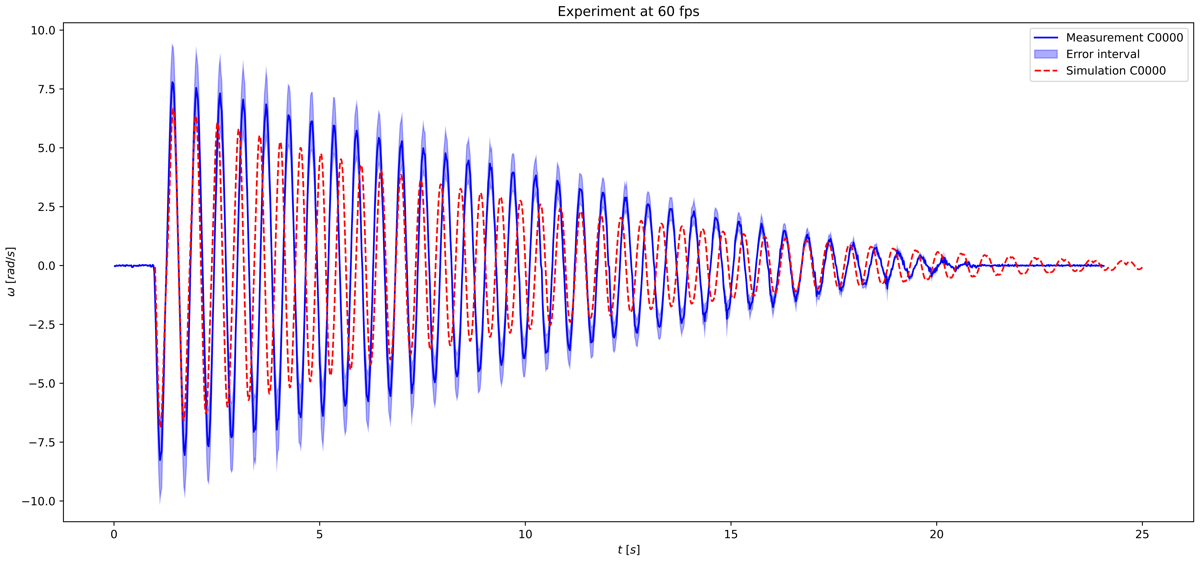
\includegraphics[width=\textwidth]{exp_C0000.png}
    \centering
    \caption{Porovnání měření a simulace experimentu C0000 (60 fps)}
    \label{fig:exp_C0000}
\end{figure}

Výsledné porovnání v grafu \ref{fig:exp_C0000} je velmi uspokojivé. Vidíme, že amplituda i frekvence jsou velmi podobné v průběhu celého měření. Mezi možné důvody, proč simulace neodpovídá měření více, patří například: další vibrace a jiné nechtěné jevy v ložisku; nepřesné určení třecích koeficientů; nepřesnost popisu velkého magnetu v simulaci pomocí několika magnetických momentů.

\clearpage

\subsection{Výsledky měření při 1000fps}

Další tři měření se zaměřují na mikroskopické chování, a to za různých rychlostí - experiment C0002 je za vysokých otáček, experiment C0004 za nižších otáček a v experimentu C0007 spinner osciluje kolem rovnovážné polohy stejně jako v experimentu C0000.

\begin{figure}[!ht]
    % \vspace*{0.75cm}
    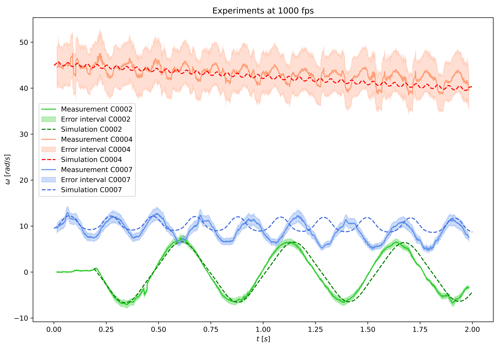
\includegraphics[width=\textwidth]{exp_C000247.png}
    \centering
    \caption{Porovnání měření a simulace experimentů C0002, C0004 a C0007 (1000 fps)}
    \label{fig:exp_C000247}
\end{figure}

Graf \ref{fig:exp_C000247} ukazuje, že s rostoucí rychlostí se měření a simulace více a více rozcházejí. Toto může opět být způsobeno nechtěnými jevy, jako například vibracemi v ložisku, které mohou být při vyšších rychlostech více prominentní. Při nižších otáčkách stále sledujeme velmi dobrou shodu frekvencí a amplitud. Simulování vysokých rychlostí jsme tedy označili za možnou slabinu naší simulace.